\documentclass[
    hyperref={bookmarks=false},% ,, linkcolor=blue, urlcolor=blue,, colorlinks=true, citecolor=MidnightBlue
    xcolor={dvipsnames},
]{beamer}

\usetheme[height=8mm]{Rochester} % Main Theme
\usecolortheme{default} % Color Theme
\usepackage{lmodern} % Optional to remove font size warnings
\newcommand{\term}[1]{\textcolor{Mahogany}{#1}}

\usefonttheme[onlymath]{serif} % For serif font in math mode

\usepackage{../../packages/shared}
\usepackage{../../packages/misc_commands}
% =========================
% Causal Structure Diagrams
% =========================
\definecolor{obs_outline}{RGB}{51,157,215}
\definecolor{obs_fill}{RGB}{222,253,255}
\definecolor{obs_text}{RGB}{0,0,0}
\definecolor{lat_outline}{RGB}{251,141,54}
\definecolor{cause}{RGB}{30, 0, 30}
\definecolor{lat_fill}{RGB}{255,213,153}
\definecolor{lat_text}{RGB}{0,0,0}
\tikzset{square/.style={regular polygon,regular polygon sides=4}}
\tikzset{triangle/.style={regular polygon,regular polygon sides=3}}
\tikzset{observed/.style={obs_text, triangle, thick, draw=obs_outline, fill=obs_fill, inner sep=0em, minimum size=3em}}
\tikzset{latent/.style={lat_text, circle, thick, draw=lat_outline, fill=lat_fill}}
% \tikzset{cause/.style={mid arrow/.style={postaction={decorate,decoration={markings, mark=at position .5 with {\arrow[#1]{stealth}}}}},}}
\tikzset{
    % style to apply some styles to each segment of a path
    on each segment/.style={
        decorate,
        decoration={
            show path construction,
            moveto code={},
            lineto code={
                \path [#1]
                (\tikzinputsegmentfirst) -- (\tikzinputsegmentlast);
            },
            curveto code={
                \path [#1] (\tikzinputsegmentfirst)
                .. controls
                (\tikzinputsegmentsupporta) and (\tikzinputsegmentsupportb)
                ..
                (\tikzinputsegmentlast);
            },
            closepath code={
                \path [#1]
                (\tikzinputsegmentfirst) -- (\tikzinputsegmentlast);
            },
        },
    },
    % style to add an arrow in the middle of a path
    mid arrow/.style={postaction={decorate,decoration={
                markings,
                mark=at position .6 with {\arrow[scale=1.5, cause]{stealth}}
            }}},
}
% =========================
% ========================= % Causal structure formatting for tikz

\title[Inflation Technique]{Inflation Technique}
\author[]{A Brief Introduction}
\date[]{2016}

\begin{document}

\begin{frame}
    \titlepage
\end{frame}

\begin{frame}
    \frametitle{Graph Theory Notation}
    Let $n, m \in \nodes$ be nodes of the graph $\graph$.
    \begin{itemize}
        \item \term{parents of $n$}: $\Pa[\graph]{n} \defined \bc{m \mid m \to n}$
        \item \term{children of $n$}: $\Ch[\graph]{n} \defined \bc{m \mid n \to m}$
        \item \term{ancestry of $n$}: $\An[\graph]{n} \defined \bigcup_{i\in\mathbb{W}} \Pa[\graph][i]{n}$
    \end{itemize}
    \[ \Pa[\graph][0]{n} = n \qquad \Pa[\graph][i]{n} \defined \Pa[\graph]{\Pa[\graph][i-1]{n}} \]
    Notation extends to sets of nodes $N \subseteq \nodes$,
    \begin{itemize}
        \item \term{parents of $N$}: $\Pa[\graph]{N} \defined \bigcup_{n\in N}\Pa[\graph]{n}$
        \item \term{children of $N$}: $\Ch[\graph]{N} \defined \bigcup_{n\in N}\Ch[\graph]{n}$
        \item \term{ancestry of $N$}: $\An[\graph]{N} \defined \bigcup_{n\in N}\An[\graph]{n}$
    \end{itemize}
    An \term{induced subgraph} of $\graph = \br{\nodes, \edges}$ due to $N \subseteq \nodes$
    \[ \Sub[\graph]{N} = \br{N, \bc{e \in \edges \mid e \subseteq N}} \]
\end{frame}

\begin{frame}
    \frametitle{Inflation Technique}
    \begin{definition}
        An \term{inflation} of a causal structure $\graph$ is another causal structure $\graph'$ such that:
        \[ \forall n' \in \nodes', n' \sim n \in \nodes: \AnSub[\graph']{n'} \sim \AnSub[\graph]{n} \]
        Where $\AnSub[\graph]{n}$ denotes the \term{ancestral sub-graph} of $n$ in $\graph$
        \[ \AnSub[\graph]{n} = \Sub[\graph]{\An[\graph]{n}} \]
        And '$\sim$' is a \term{copy-index} equivalence relation
        \[ A_1 \sim A_2 \sim A \not \sim B_1 \sim B_2 \sim B \]
    \end{definition}
\end{frame}

\begin{frame}
    \frametitle{Case Study: The Triangle Scenario}
    \begin{center}
        \scalebox{1.5}{\begin{tikzpicture}[scale=1]
    \begin{scope}[every node/.style=observed]
        \node (C) at (-2, 0) {$C$};
        \node (B) at (2, 0) {$B$};
        \node (A) at (0, {2*sqrt(3)}) {$A$};
    \end{scope}
    \begin{scope}[every node/.style=latent]
        \node (X) at (-1, {sqrt(3)}) {$X$};
        \node (Y) at (1, {sqrt(3)}) {$Y$};
        \node (Z) at (0, 0) {$Z$};
    \end{scope}
    \begin{scope}[every path/.style={draw=cause, thick}]
        \path[postaction={on each segment={mid arrow}}]
        (X) -- (A)
        (X) -- (C)
        (Y) -- (A)
        (Y) -- (B)
        (Z) -- (B)
        (Z) -- (C);
    \end{scope}
\end{tikzpicture}}
    \end{center}
\end{frame}

\begin{frame}
    \frametitle{Some Inflations of the Triangle Scenario}
    \begin{center}
    \begin{tabular}{cc}
        %\hline
        \scalebox{0.4}{\newcommand{\ift}{2.3}
\newcommand{\hvspoke}{0.8}
\newcommand{\diagspoke}{1.1}
\begin{tikzpicture}[scale=2]
    \begin{scope}[every node/.style=observed]
        \node (A1) at ({0}, {\hvspoke}) {$\p{A}_1$};
        \node (A2) at ({0}, {-\hvspoke}) {$\p{A}_2$};
        \node (B1) at ({-\hvspoke}, {0}) {$\p{B}_1$};
        \node (B2) at ({\hvspoke}, {0}) {$\p{B}_2$};
        \node (C1) at ({+\diagspoke}, {+\diagspoke}) {$\p{C}_1$};
        \node (C2) at ({+\diagspoke}, {-\diagspoke}) {$\p{C}_2$};
        \node (C3) at ({-\diagspoke}, {-\diagspoke}) {$\p{C}_3$};
        \node (C4) at ({-\diagspoke}, {+\diagspoke}) {$\p{C}_4$};
    \end{scope}
    \begin{scope}[every node/.style=latent]
        \node (Y1) at (0, 0) {$\p{Y}_1$};
        \node (X1) at ({0}, {2*\hvspoke}) {$\p{X}_1$};
        \node (Z1) at ({2*\hvspoke}, {0}) {$\p{Z}_1$};
        \node (X2) at ({0}, {-2*\hvspoke}) {$\p{X}_2$};
        \node (Z2) at ({-2*\hvspoke}, {0}) {$\p{Z}_2$};
    \end{scope}
    \begin{scope}[every path/.style={draw=cause, thick}]
        \path[postaction={on each segment={mid arrow}}]
        % Y1
        (Y1) -- (A1)
        (Y1) -- (A2)
        (Y1) -- (B1)
        (Y1) -- (B2)
        % X1
        (X1) -- (C1)
        (X1) -- (C4)
        (X1) -- (A1)
        % Z1
        (Z1) -- (C1)
        (Z1) -- (C2)
        (Z1) -- (B2)
        % X2
        (X2) -- (C2)
        (X2) -- (C3)
        (X2) -- (A2)
        % Z2
        (Z2) -- (C4)
        (Z2) -- (C3)
        (Z2) -- (B1)
        ;
    \end{scope}
\end{tikzpicture}}
        &
        \scalebox{0.5}{\newcommand{\ift}{2.3}
\begin{tikzpicture}[scale=2]
    \begin{scope}[every node/.style=observed]
        \node (C2) at ({-2 + 2*1/\ift}, {2*1/(\ift*sqrt(3))}) {$C_2$};
        \node (C1) at ({-2 + 3*1/\ift}, {3*1/(\ift*sqrt(3))}) {$C_1$};
        \node (B2) at ({2 - 2*1/\ift}, {2*1/(\ift*sqrt(3))}) {$B_2$};
        \node (B1) at ({2 - 3*1/\ift}, {3*1/(\ift*sqrt(3))}) {$B_1$};
        \node (A2) at (0, {2*sqrt(3) - 2*2/sqrt(3)*(1/\ift)}) {$A_2$};
        \node (A1) at (0, {2*sqrt(3) - 3*2/sqrt(3)*(1/\ift)}) {$A_1$};
    \end{scope}
    \begin{scope}[every node/.style=latent]
        \node (X2) at (-1, {sqrt(3)}) {$X_2$};
        \node (X1) at ({-1 + 1/\ift}, {sqrt(3) - 1/(\ift*sqrt(3))}) {$X_1$};
        \node (Y2) at (1, {sqrt(3)}) {$Y_2$};
        \node (Y1) at ({1 - 1/\ift}, {sqrt(3) - 1/(\ift*sqrt(3))}) {$Y_1$};
        \node (Z1) at (0, 0.5) {$Z_1$};
        \node (Z2) at (0, 0) {$Z_2$};
    \end{scope}
    \begin{scope}[every path/.style={draw=cause, thick}]
        \path[postaction={on each segment={mid arrow}}]
        (X1) -- (A1) (X1) -- (C1) (X2) -- (C2) (X1) -- (A2)
        (Y1) -- (A1) (Y1) -- (B1) (Y2) -- (A2) (Y1) -- (B2)
        (Z1) -- (B1) (Z1) -- (C1) (Z2) -- (B2) (Z1) -- (C2)
        ;
    \end{scope}
\end{tikzpicture}}
        \\
        %\hline
        Wagon Wheel Inflation
        &
        Spiral Inflation \\
        %\hline
        \scalebox{0.5}{\newcommand{\ift}{2.3}
\begin{tikzpicture}[scale=2]
    \begin{scope}[every node/.style=observed]
        \node (C1) at ({-2 + 3*1/\ift}, {3*1/(\ift*sqrt(3))}) {$C_1$};
        \node (B1) at ({2 - 3*1/\ift}, {3*1/(\ift*sqrt(3))}) {$B_1$};
        \node (A1) at (0, {2*sqrt(3) - 2*2/sqrt(3)*(1/\ift)}) {$A_1$};
    \end{scope}
    \begin{scope}[every node/.style=latent]
        \node (X1) at ({-1 + 1/\ift}, {sqrt(3) - 1/(\ift*sqrt(3))}) {$X_1$};
        \node (Y2) at (1, {sqrt(3)}) {$Y_2$};
        \node (Y1) at ({1 - 1/\ift}, {sqrt(3) - 1/(\ift*sqrt(3))}) {$Y_1$};
        \node (Z1) at (0, 0.5) {$Z_1$};
    \end{scope}
    \begin{scope}[every path/.style={draw=cause, thick}]
        \path[postaction={on each segment={mid arrow}}]
        (X1) -- (A1) (X1) -- (C1)
        (Y2) -- (A1) (Y1) -- (B1)
        (Z1) -- (B1) (Z1) -- (C1)
        ;
    \end{scope}
\end{tikzpicture}}
        &
        \scalebox{0.5}{\newcommand{\ift}{2.3}
\begin{tikzpicture}[scale=2]
    \begin{scope}[every node/.style=observed]
        \node (C4) at (-2, 0) {$C_4$};
        \node (C3) at ({-2 + 1/\ift}, {1/(\ift*sqrt(3))}) {$C_3$};
        \node (C2) at ({-2 + 2*1/\ift}, {2*1/(\ift*sqrt(3))}) {$C_2$};
        \node (C1) at ({-2 + 3*1/\ift}, {3*1/(\ift*sqrt(3))}) {$C_1$};
        \node (B4) at (2, 0) {$B_4$};
        \node (B3) at ({2 - 1/\ift}, {1/(\ift*sqrt(3))}) {$B_3$};
        \node (B2) at ({2 - 2*1/\ift}, {2*1/(\ift*sqrt(3))}) {$B_2$};
        \node (B1) at ({2 - 3*1/\ift}, {3*1/(\ift*sqrt(3))}) {$B_1$};
        \node (A4) at (0, {2*sqrt(3)}) {$A_4$};
        \node (A3) at (0, {2*sqrt(3) - 2/sqrt(3)*(1/\ift)}) {$A_3$};
        \node (A2) at (0, {2*sqrt(3) - 2*2/sqrt(3)*(1/\ift)}) {$A_2$};
        \node (A1) at (0, {2*sqrt(3) - 3*2/sqrt(3)*(1/\ift)}) {$A_1$};
    \end{scope}
    \begin{scope}[every node/.style=latent]
        \node (X2) at (-1, {sqrt(3)}) {$X_2$};
        \node (X1) at ({-1 + 1/\ift}, {sqrt(3) - 1/(\ift*sqrt(3))}) {$X_1$};
        \node (Y2) at (1, {sqrt(3)}) {$Y_2$};
        \node (Y1) at ({1 - 1/\ift}, {sqrt(3) - 1/(\ift*sqrt(3))}) {$Y_1$};
        \node (Z1) at (0, 0.5) {$Z_1$};
        \node (Z2) at (0, 0) {$Z_2$};
    \end{scope}
    \begin{scope}[every path/.style={draw=cause, thick}]
        \path[postaction={on each segment={mid arrow}}]
        (X2) -- (A4) (X2) -- (C4) (X2) -- (C2) (X2) -- (A3)
        (Y2) -- (A4) (Y2) -- (B4) (Y2) -- (A2) (Y2) -- (B3)
        (Z2) -- (B4) (Z2) -- (C4) (Z2) -- (B2) (Z2) -- (C3)
        (X1) -- (A1) (X1) -- (C1) (X1) -- (C3) (X1) -- (A2)
        (Y1) -- (A1) (Y1) -- (B1) (Y1) -- (A3) (Y1) -- (B2)
        (Z1) -- (B1) (Z1) -- (C1) (Z1) -- (B3) (Z1) -- (C2)
        ;
    \end{scope}
\end{tikzpicture}}
        \\
        %\hline
        Cut Inflation
        &
        Web Inflation \\
        %\hline
    \end{tabular}
    \end{center}
\end{frame}

\begin{frame}
    \frametitle{Demonstrating Inflation Technique}
    \vfill
    \begin{center}
    \begin{columns}
        \column{0.5\linewidth}%
        \scalebox{1.0}{\begin{tikzpicture}[scale=1]
    \begin{scope}[every node/.style=observed, onslide=<2->{fade}]
        \node[onslide=<3>{unfade}] (C) at (-2, 0) {$\p{C}$};
        \node (B) at (2, 0) {$\p{B}$};
        \node[onslide=<2>{unfade}] (A) at (0, {2*sqrt(3)}) {$\p{A}$};
    \end{scope}
    \begin{scope}[every node/.style=latent, onslide=<2->{fade}]
        \node[onslide=<2-3>{unfade}] (X) at (-1, {sqrt(3)}) {$\p{X}$};
        \node[onslide=<2>{unfade}] (Y) at (1, {sqrt(3)}) {$\p{Y}$};
        \node[onslide=<3>{unfade}] (Z) at (0, 0) {$\p{Z}$};
    \end{scope}
    \begin{scope}[every path/.style={draw=cause, thick}, onslide=<2->{fade}]
        \path[postaction={on each segment={mid arrow}}]
        (Y) -- (B)
        (Z) -- (B)
        ;
        \path[postaction={on each segment={mid arrow}}, onslide=<3>{unfade}]
        (X) -- (C)
        (Z) -- (C)
        ;
        \path[postaction={on each segment={mid arrow}}, onslide=<2>{unfade}]
        (X) -- (A)
        (Y) -- (A)
        ;
    \end{scope}
\end{tikzpicture}}
        \column{0.5\linewidth}%
        \scalebox{1.0}{\input{../../figures/causal_structures/inflated_triangle_scenario_spiral_anim_1}}
    \end{columns}
    \end{center}
    \only<1>{\[\forall n' \in \nodes', n' \sim n \in \nodes: \AnSub[\graph']{n'} \sim \AnSub[\graph]{n}\]}%
    \only<2>{\[\AnSub[\graph]{A} \sim \AnSub[\graph']{A_1}\]}%
    \only<3>{\[\AnSub[\graph]{C} \sim \AnSub[\graph']{C_2}\]}%
\end{frame}


\begin{frame}
    \frametitle{What are Injectable Sets?}
    \begin{center}
    \begin{columns}
        \column{0.5\linewidth}%
        \scalebox{1.0}{\begin{tikzpicture}[scale=1]
    \draw[red,scale=2, transform shape, onslide=<1>{opacity=0}, onslide=<2>{unfade}] (0,{0.7}) node{\textbf{\Huge ?}};
    \begin{scope}[every node/.style=observed, onslide=<1->{fade}]
        \node[onslide=<1>{unfade}] (C) at (-2, 0) {$\p{C}$};
        \node (B) at (2, 0) {$\p{B}$};
        \node[onslide=<1>{unfade}] (A) at (0, {2*sqrt(3)}) {$\p{A}$};
    \end{scope}
    \begin{scope}[every node/.style=latent, onslide=<1->{fade}]
        \node[onslide=<1>{unfade}] (X) at (-1, {sqrt(3)}) {$\p{X}$};
        \node[onslide=<1>{unfade}] (Y) at (1, {sqrt(3)}) {$\p{Y}$};
        \node[onslide=<1>{unfade}] (Z) at (0, 0) {$\p{Z}$};
    \end{scope}
    \begin{scope}[every path/.style={draw=cause, thick}, onslide=<1->{fade}]
        \path[postaction={on each segment={mid arrow}}]
        (Y) -- (B)
        (Z) -- (B)
        ;
        \path[postaction={on each segment={mid arrow}}, onslide=<1>{unfade}]
        (X) -- (C)
        (Z) -- (C)
        ;
        \path[postaction={on each segment={mid arrow}}, onslide=<1>{unfade}]
        (X) -- (A)
        (Y) -- (A)
        ;
    \end{scope}
\end{tikzpicture}}
        \column{0.5\linewidth}%
        \scalebox{1.0}{\newcommand{\ift}{2.3}
\begin{tikzpicture}[scale=2]
    \begin{scope}[every node/.style=observed, onslide=<1->{fade}]
        \node[onslide=<3>{unfade}] (C2) at ({-2 + 2*1/\ift}, {2*1/(\ift*sqrt(3))}) {$C_2$};
        \node[onslide=<1>{unfade}] (C1) at ({-2 + 3*1/\ift}, {3*1/(\ift*sqrt(3))}) {$C_1$};
        \node[onslide=<2>{unfade},onslide=<3>{unfade}] (B2) at ({2 - 2*1/\ift}, {2*1/(\ift*sqrt(3))}) {$B_2$};
        \node[onslide=<2>{unfade}] (B1) at ({2 - 3*1/\ift}, {3*1/(\ift*sqrt(3))}) {$B_1$};
        \node[onslide=<1>{unfade}] (A2) at (0, {2*sqrt(3) - 2*2/sqrt(3)*(1/\ift)}) {$A_2$};
        \node[] (A1) at (0, {2*sqrt(3) - 3*2/sqrt(3)*(1/\ift)}) {$A_1$};
    \end{scope}
    \begin{scope}[every node/.style=latent, onslide=<1->{fade}]
        \node[onslide=<3>{unfade}] (X2) at (-1, {sqrt(3)}) {$X_2$};
        \node[onslide=<1>{unfade}] (X1) at ({-1 + 1/\ift}, {sqrt(3) - 1/(\ift*sqrt(3))}) {$X_1$};
        \node[onslide=<1>{unfade}] (Y2) at (1, {sqrt(3)}) {$Y_2$};
        \node[onslide=<2>{unfade}, onslide=<3>{unfade}] (Y1) at ({1 - 1/\ift}, {sqrt(3) - 1/(\ift*sqrt(3))}) {$Y_1$};
        \node[onslide=<1>{unfade}, onslide=<2>{unfade}, onslide=<3>{unfade}] (Z1) at (0, 0.5) {$Z_1$};
        \node[onslide=<2>{unfade}, onslide=<3>{unfade}] (Z2) at (0, 0) {$Z_2$};
    \end{scope}
    \begin{scope}[every path/.style={draw=cause, thick}, onslide=<1->{fade}]
        \path[postaction={on each segment={mid arrow}}, onslide=<2>{unfade}, onslide=<3>{unfade}]
        (Y1) -- (B2) (Z2) -- (B2)
        ;
        \path[postaction={on each segment={mid arrow}}, onslide=<2>{unfade}]
        (Y1) -- (B1) (Z1) -- (B1)
        ;
        \path[postaction={on each segment={mid arrow}}, onslide=<1>{unfade}]
        (X1) -- (A2) (X1) -- (C1) (Z1) -- (C1) (Y2) -- (A2)
        ;
        \path[postaction={on each segment={mid arrow}}, onslide=<3>{unfade}]
        (X2) -- (C2) (Z1) -- (C2)
        ;
        \path[postaction={on each segment={mid arrow}}, ]
        (Y1) -- (A1) (X1) -- (A1)
        ;
    \end{scope}
\end{tikzpicture}}
    \end{columns}
    \end{center}
    \only<1>{\[\AnSub[\graph]{A,C} \sim \AnSub[\graph']{A_2,C_1}\]}%
    \only<2>{\[?? \not \sim \AnSub[\graph']{B_1,B_2}\]}%
    \only<3>{\[?? \not \sim \AnSub[\graph']{B_2,C_2}\]}%
\end{frame}

\begin{frame}
    \frametitle{Injectable Sets Defined}
    \vfill
    The \term{injectable sets in $\graph'$}:
    \begin{align*}
        \Inj[\graph]{\graph'} &\defined \bc{N' \subseteq \nodes' \mid \exists N \subseteq \nodes : N \sim N'}
    \end{align*}
    The \term{images of the injectable sets in $\graph$}:
    \begin{align*}
        \ImInj[\graph]{\graph'} &\defined \bc{N \subseteq \nodes \mid \exists N' \subseteq \nodes' : N \sim N'}
    \end{align*}
    \vfill
    \begin{center}
        \textbf{What makes injectable sets useful?}
    \end{center}
    \vfill
\end{frame}

\begin{frame}
    \frametitle{Inflation Lemma}
    \begin{lemma}[Inflation Lemma]
    Given $\graph = \br{\nodes, \edges}$ and inflation $\graph' = \br{\nodes', \edges'}$:
    \begin{center}
        \begin{tikzpicture}
            \pgfmathsetmacro{\vs}{2.2};
            \pgfmathsetmacro{\hs}{5.2};
            \draw (0*\hs,0*\vs) node[](pn){$\underbrace{\bc{\prob[N] \mid N \in \ImInj[\graph]{\graph'}}}_{\text{compatible with $\graph$}}$};
            \draw (1*\hs,0*\vs) node[](cp){$\bc{\prob[n\mid \Pa[\graph]{n}] \mid n \in \nodes}$};
            \draw (1*\hs,-1*\vs) node[](cp_){$\bc{\prob[n'\mid \Pa[\graph']{n'}] \mid n' \in \nodes'}$};
            \draw (0*\hs,-1*\vs) node[](pn_){$\underbrace{\bc{\prob[N'] \mid N' \in \Inj[\graph]{\graph'}}}_{\text{compatible with $\graph'$}}$};
            \draw[very thick, ->] (pn) -- (cp);
            \draw[very thick, ->] (cp) -- (cp_) node [midway, above, sloped]{{\footnotesize define}};
            \draw[very thick, ->] (cp_) -- (pn_);
        \end{tikzpicture}
    \end{center}
    \end{lemma}
    \begin{corollary}
        All inequalities $I'$ constraining $\Inj[\graph]{\graph'}$ can be \term{deflated} into inequalities $I$ constraining $\ImInj[\graph]{\graph'}$ by dropping copy-indices.
    \end{corollary}
\end{frame}

\begin{frame}
    \frametitle{Perfect Correlation Is Incompatible}
    \begin{columns}
        \column{0.5\linewidth}
        \begin{center}
            \includegraphics[width=\linewidth]{../../figures/distributions/perfect_correlation_2_outcomes.pdf}
        \end{center}
        \column{0.5\linewidth}
        \begin{align*}
        \probplotvalue{0, 0, 0} &= \f12 \\
        \prob[ABC][abc] &= \f{\bs{000} + \bs{111}}{2} \\
        \prob[ABC][abc] &= \begin{cases}
            \f12 & a = b = c \\
            0 & \text{ otherwise }
        \end{cases}
        \end{align*}
    \end{columns}
    \begin{center}
        Compatibility Inequality
    \end{center}
    \[ \prob[A][0]\prob[B][1] \leq \prob[BC][10] + \prob[AC][01] \]
    \begin{center}
        Witnesses Perfect Correlation
    \end{center}
    \[ \br{\f{1}{2}}^{2} \not\leq 0 + 0 \]
\end{frame}
\makeatletter
\renewcommand*\env@matrix[1][*\c@MaxMatrixCols c]{%
  \hskip -\arraycolsep
  \let\@ifnextchar\new@ifnextchar
  \array{#1}}
\makeatother
\begin{frame}
    \frametitle{Deriving Compatibility Inequalities}
    \begin{center}
        \scalebox{0.8}{\newcommand{\ift}{2.3}
\begin{tikzpicture}[scale=2]
    \begin{scope}[every node/.style=observed]
        \node (C1) at ({-2 + 3*1/\ift}, {3*1/(\ift*sqrt(3))}) {$C_1$};
        \node (B1) at ({2 - 3*1/\ift}, {3*1/(\ift*sqrt(3))}) {$B_1$};
        \node (A1) at (0, {2*sqrt(3) - 2*2/sqrt(3)*(1/\ift)}) {$A_1$};
    \end{scope}
    \begin{scope}[every node/.style=latent]
        \node (X1) at ({-1 + 1/\ift}, {sqrt(3) - 1/(\ift*sqrt(3))}) {$X_1$};
        \node (Y2) at (1, {sqrt(3)}) {$Y_2$};
        \node (Y1) at ({1 - 1/\ift}, {sqrt(3) - 1/(\ift*sqrt(3))}) {$Y_1$};
        \node (Z1) at (0, 0.5) {$Z_1$};
    \end{scope}
    \begin{scope}[every path/.style={draw=cause, thick}]
        \path[postaction={on each segment={mid arrow}}]
        (X1) -- (A1) (X1) -- (C1)
        (Y2) -- (A1) (Y1) -- (B1)
        (Z1) -- (B1) (Z1) -- (C1)
        ;
    \end{scope}
\end{tikzpicture}}
    \end{center}
    \[ \mscenario = \bc{\bc{A_1, B_1}, \bc{B_1, C_1}, \bc{A_1, C_1}} \]
    \[ \prob^{\mscenario} = \bc{\prob[A_1B_1], \prob[B_1C_1], \prob[A_1C_1]} \]
    \[ \text{Compatibility requires:} \qquad \exists \prob[\jointvar] = \prob[A_1B_1C_1] \]
    \[ \prob[A_1B_1] = {\sum}_{C_1} \prob[\jointvar] \qquad \prob[B_1C_1] = {\sum}_{A_1} \prob[\jointvar] \qquad \prob[A_1C_1] = {\sum}_{B_1} \prob[\jointvar]\]
\end{frame}

\begin{frame}[shrink=13]
    \frametitle{Deriving Compatibility Inequalities Cont'd}
    \[ \underbrace{\prob[A_1B_1] = {\sum}_{C_1} \prob[\jointvar] \qquad \prob[B_1C_1] = {\sum}_{A_1} \prob[\jointvar] \qquad \prob[A_1C_1] = {\sum}_{B_1} \prob[\jointvar]} \]
    \[ \underbrace{\forall V \in \mscenario: \prob[V] = \sum_{\jointvar \setminus V} \prob[\jointvar] }\]
    \[ \probvec^{\mscenario} = M \tcdot \probvec^{\jointvar}  \]
    \[ \probvec^{\mscenario} =
        \begin{pmatrix}
            \prob[A_1B_1][00] \\
            \prob[A_1B_1][01] \\
            \prob[A_1B_1][10] \\
            \prob[A_1B_1][11] \\
            \hline
            \prob[B_1C_1][00] \\
            \prob[B_1C_1][01] \\
            \prob[B_1C_1][10] \\
            \prob[B_1C_1][11] \\
            \hline
            \prob[A_1C_1][00] \\
            \prob[A_1C_1][01] \\
            \prob[A_1C_1][10] \\
            \prob[A_1C_1][11] \\
        \end{pmatrix}
        \qquad
        \probvec^{\jointvar} =
        \begin{pmatrix}
            \prob[A_1B_1C_1][000] \\
            \prob[A_1B_1C_1][001] \\
            \prob[A_1B_1C_1][010] \\
            \prob[A_1B_1C_1][011] \\
            \prob[A_1B_1C_1][100] \\
            \prob[A_1B_1C_1][101] \\
            \prob[A_1B_1C_1][110] \\
            \prob[A_1B_1C_1][111] \\
        \end{pmatrix}
    \]
\end{frame}

\begin{frame}[shrink=15]
    \frametitle{Incidence Example}
    \[ M = \kbordermatrix{
        (A_1,B_1,C_1) \:\: = & (0,0,0) & (0,0,1) & (0,1,0) & (0,1,1) & (1,0,0) & (1,0,1) & (1,1,0) & (1,1,1) \\
        (A_1=0, B_1=0) & \kone & \kone & \kzer & \kzer & \kzer & \kzer & \kzer & \kzer \\
        (A_1=0, B_1=1) & \kzer & \kzer & \kone & \kone & \kzer & \kzer & \kzer & \kzer \\
        (A_1=1, B_1=0) & \kzer & \kzer & \kzer & \kzer & \kone & \kone & \kzer & \kzer \\
        (A_1=1, B_1=1) & \kzer & \kzer & \kzer & \kzer & \kzer & \kzer & \kone & \kone \\
        (B_1=0, C_1=0) & \kone & \kzer & \kzer & \kzer & \kone & \kzer & \kzer & \kzer \\
        (B_1=0, C_1=1) & \kzer & \kone & \kzer & \kzer & \kzer & \kone & \kzer & \kzer \\
        (B_1=1, C_1=0) & \kzer & \kzer & \kone & \kzer & \kzer & \kzer & \kone & \kzer \\
        (B_1=1, C_1=1) & \kzer & \kzer & \kzer & \kone & \kzer & \kzer & \kzer & \kone \\
        (A_1=0, C_1=0) & \kone & \kzer & \kone & \kzer & \kzer & \kzer & \kzer & \kzer \\
        (A_1=0, C_1=1) & \kzer & \kone & \kzer & \kone & \kzer & \kzer & \kzer & \kzer \\
        (A_1=1, C_1=0) & \kzer & \kzer & \kzer & \kzer & \kone & \kzer & \kone & \kzer \\
        (A_1=1, C_1=1) & \kzer & \kzer & \kzer & \kzer & \kzer & \kone & \kzer & \kone
    } \]
    \[ \probvec^{\mscenario} = M \tcdot \probvec^{\jointvar}  \]
\end{frame}

\begin{frame}
    \frametitle{Finding Inequalities}
    \begin{columns}[T]
        \column{0.4\linewidth}%
            \term{Linear Program}:%
            \begin{alignat*}{2}
                & \text{minimize:} \quad&& \emptyset \tcdot x\\
                & \text{subject to:} && \probvec^{\jointvar} \succeq 0 \\
                & && M \tcdot \probvec^{\jointvar} = \probvec^{\mscenario} \\
            \end{alignat*}%
        \column{0.4\linewidth}%
            \term{Dual Linear Program}:%
            \begin{alignat*}{2}
                & \text{minimize:} \quad&& y \tcdot \probvec^{\mscenario}\\
                & \text{subject to:} && y \tcdot M \succeq 0 \\
            \end{alignat*}%
    \end{columns}
    Alternatively,
    \begin{itemize}
        \item Linear Quantifier Elimination \
        \item Fourier-Motzkin
        \item Polytope Description
        \item etc.
    \end{itemize}
\end{frame}


\begin{frame}
    \frametitle{Deflating Inequalities}
    \begin{columns}
        \column{0.5\linewidth}
            \scalebox{1.0}{\newcommand{\ift}{2.3}
\begin{tikzpicture}[scale=2]
    \begin{scope}[every node/.style=observed, onslide=<2->{fade}]
        \node (C1) at ({-2 + 3*1/\ift}, {3*1/(\ift*sqrt(3))}) {$\p{C}_1$};
        \node[onslide=<2->{unfade}] (B1) at ({2 - 3*1/\ift}, {3*1/(\ift*sqrt(3))}) {$\p{B}_1$};
        \node[onslide=<2->{unfade}] (A1) at (0, {2*sqrt(3) - 2*2/sqrt(3)*(1/\ift)}) {$\p{A}_1$};
    \end{scope}
    \begin{scope}[every node/.style=latent, onslide=<2->{fade}]
        \node[onslide=<2->{unfade}] (X1) at ({-1 + 1/\ift}, {sqrt(3) - 1/(\ift*sqrt(3))}) {$\p{X}_1$};
        \node[onslide=<2->{unfade}] (Y2) at (1, {sqrt(3)}) {$\p{Y}_2$};
        \node[onslide=<2->{unfade}] (Y1) at ({1 - 1/\ift}, {sqrt(3) - 1/(\ift*sqrt(3))}) {$\p{Y}_1$};
        \node[onslide=<2->{unfade}] (Z1) at (0, 0.5) {$\p{Z}_1$};
    \end{scope}
    \begin{scope}[every path/.style={draw=cause, thick}, onslide=<2->{fade}]
        \path[postaction={on each segment={mid arrow}}]
        (X1) -- (C1)
        (Z1) -- (C1)
        ;
        \path[postaction={on each segment={mid arrow}}, onslide=<2->{unfade}]
        (X1) -- (A1)
        (Y2) -- (A1)
        (Y1) -- (B1)
        (Z1) -- (B1)
        ;
    \end{scope}
\end{tikzpicture}}
        \column{0.5\linewidth}
            \vfill
            \begin{center}
            \[ \Inj[\graph]{\graph'} = \begin{Bmatrix}
                \bc{A_1,C_1}\\ \bc{B_1,C_1}\\ \bc{A_1}\\ \bc{B_1}\\ \bc{C_1}
            \end{Bmatrix} \]
            \[ \bc{A_1, B_1} \not \in \Inj[\graph]{\graph'} \]
            \end{center}
            \vfill
    \end{columns}
    \[ \prob[A_1B_1][01] \leq \prob[B_1C_1][10] + \prob[A_1C_1][01] \]
    \only<1>{\begin{center}\textbf{Can not deflate inequality!}\end{center}}
    \only<2>{\begin{center}\textbf{However!}\end{center}}
    \only<2>{\[ \AnSub[\graph']{A_1} \cap \AnSub[\graph']{B_1} = \emptyset \iff A_1 \ancestralindep B_1 \]}
    \onslide<3->{\[ \prob[A_1][0]\prob[B_1][1] \leq \prob[B_1C_1][10] + \prob[A_1C_1][01] \]}
    \onslide<4->{\[ \prob[A][0]\prob[B][1] \leq \prob[BC][10] + \prob[AC][01] \]}
\end{frame}

\begin{frame}
    \frametitle{Inflation Produces Polynomial Inequalities}
    \begin{itemize}
        \item Deflation demands inequality constrains injectable probabilities $\prob[N'], N' \in \Inj[\graph]{\graph'}$
        \item \textbf{Linear inequality} for $\graph'$
    \end{itemize}
    \begin{center}
        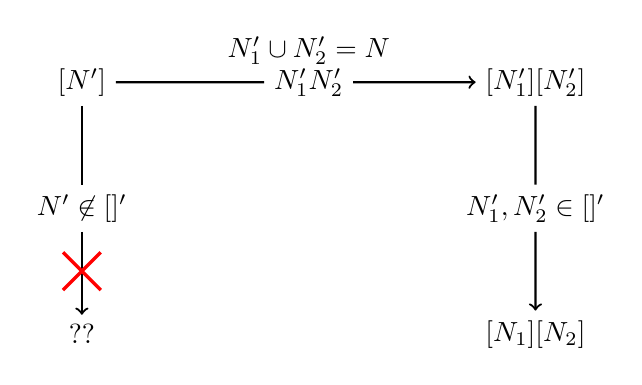
\begin{tikzpicture}[scale=0.8]
            \pgfmathsetmacro{\hs}{1.8};
            \pgfmathsetmacro{\vs}{1};
            \pgfmathsetmacro{\cross}{0.3};
            \draw (0*\hs, 4*\vs) node[](a){$\prob[N']$};
            \draw (0*\hs, 2*\vs) node[](ab){$N' \not \in \Inj[\graph]{\graph'}$};
            \draw (4*\hs, 4*\vs) node[](c){$\prob[N_1']\prob[N_2']$};
            \draw (2*\hs, 4*\vs) node[](ac){$N_1' \ancestralindep N_2'$};
            \draw (2*\hs, 4*\vs + 0.5*\vs) node[]{$N_1' \cup N_2' = N$};
            \draw (4*\hs, 2*\vs) node[](cd){$N_1', N_2' \in \Inj[\graph]{\graph'}$};
            \draw (4*\hs, 0*\vs) node[](d){$\prob[N_1]\prob[N_2]$};
            \draw (0, 0) node[](b){??};
            \draw[thick, ] (a) -- (ab);
            \draw[thick, ] (c) -- (cd);
            \draw[thick, ] (a) -- (ac);
            \draw[thick, ->] (ac) -- (c);
            \draw[thick, ->] (ab) -- (b);
            \draw[thick, ->] (cd) -- (d);
            \draw[very thick, red]
            (+ \cross, 1*\vs + \cross) -- (- \cross, 1*\vs - \cross)
            (+ \cross, 1*\vs - \cross) -- (- \cross, 1*\vs + \cross)
            ;
        \end{tikzpicture}
    \end{center}
    \begin{itemize}
        \item \textbf{Polynomial inequality} for $\graph$!
    \end{itemize}
\end{frame}

\begin{frame}
    \frametitle{Expressible Sets}
    \begin{gather*}
        \text{$d$-separation relations on $\graph'$} \\
        + \\
        \text{inequalities for $\graph'$} \\
        = \\
        \text{polynomial inequalities for $\graph$}
    \end{gather*}
\end{frame}

\end{document}